% !TeX program = pdflatex
% !BIB program = bibtex
% Template LaTeX file for DAFx-19 papers

%------------------------------------------------------------------------------------------
%  !  !  !  !  !  !  !  !  !  !  !  ! user defined variables  !  !  !  !  !  !  !  !  !  !  !  !  !  !
% Please use these commands to define title and author(s) of the paper:
\def\papertitle{Waterbottle Synthesis with Modal Signal Processing}
\def\paperauthorA{Jatin Chowdhury, Mark Rau, and Elliot K. Canfield-Dafilou}

% Authors' affiliations have to be set below

%------------------------------------------------------------------------------------------
\documentclass[twoside,a4paper]{article}
\usepackage{etoolbox}
\usepackage{dafx_20}
\usepackage{amsmath,amssymb,amsfonts,amsthm}
\usepackage{euscript}
\usepackage[latin1]{inputenc}
\usepackage[T1]{fontenc}
\usepackage{ifpdf}

\usepackage[english]{babel}
\usepackage{caption}
\usepackage{subfig} % or can use subcaption package
\usepackage{xcolor}

\input glyphtounicode
\pdfgentounicode=1

\setcounter{page}{1}
\ninept

% build the list of authors and set the flag \multipleauth to handle the et al. in the copyright note (in DAFx_20.sty)
%==============================DO NOT MODIFY =======================================
\newcounter{numauth}\setcounter{numauth}{1}
\newcounter{listcnt}\setcounter{listcnt}{1}
\newcommand\authcnt[1]{\ifdefined#1 \stepcounter{numauth} \fi}

\newcommand\addauth[1]{
\ifdefined#1 
\stepcounter{listcnt}
\ifnum \value{listcnt}<\value{numauth}
\appto\authorslist{, #1}
\else
\appto\authorslist{~and~#1}
\fi
\fi}
%======DO NOT MODIFY UNLESS YOUR PAPER HAS MORE THAN 10 AUTHORS========================
%==we count the authors defined at the beginning of the file (paperauthorA is mandatory and already accounted for)
\authcnt{\paperauthorB}
\authcnt{\paperauthorC}
\authcnt{\paperauthorD}
\authcnt{\paperauthorE}
\authcnt{\paperauthorF}
\authcnt{\paperauthorG}
\authcnt{\paperauthorH}
\authcnt{\paperauthorI}
\authcnt{\paperauthorJ}
%==we create a list of authors for pdf tagging, for example: paperauthorA, paperauthorB, ... and paperauthorF (last author)
\def\authorslist{\paperauthorA}
\addauth{\paperauthorB}
\addauth{\paperauthorC}
\addauth{\paperauthorD}
\addauth{\paperauthorE}
\addauth{\paperauthorF}
\addauth{\paperauthorG}
\addauth{\paperauthorH}
\addauth{\paperauthorI}
\addauth{\paperauthorJ}
%====================================================================================

\usepackage{times}
% Saves a lot of ouptut space in PDF... after conversion with the distiller
% Delete if you cannot get PS fonts working on your system.

% pdf-tex settings: detect automatically if run by latex or pdflatex
\newif\ifpdf
\ifx\pdfoutput\relax
\else
   \ifcase\pdfoutput
      \pdffalse
   \else
      \pdftrue
\fi

\ifpdf % compiling with pdflatex
  \usepackage[pdftex,
    pdftitle={\papertitle},
    pdfauthor={\paperauthorA},
    colorlinks=false, % links are activated as colror boxes instead of color text
    bookmarksnumbered, % use section numbers with bookmarks
    pdfstartview=XYZ % start with zoom=100% instead of full screen; especially useful if working with a big screen :-)
  ]{hyperref}
  \pdfcompresslevel=9
  \usepackage[pdftex]{graphicx}
%   \usepackage[figure,table]{hypcap}
\else % compiling with latex
  \usepackage[dvips]{epsfig,graphicx}
  \usepackage[dvips,
    colorlinks=false, % no color links
    bookmarksnumbered, % use section numbers with bookmarks
    pdfstartview=XYZ % start with zoom=100% instead of full screen
  ]{hyperref}
  % hyperrefs are active in the pdf file after conversion
  % \usepackage[figure,table]{hypcap}
\fi
\usepackage[hypcap=true]{caption}

% My packages
\usepackage{tikz}
\usepackage{tkz-euclide}
\usetkzobj{all}
\usepackage{cleveref}

\usepackage{listings}
\definecolor{codegreen}{rgb}{0,0.6,0}
\definecolor{codegray}{rgb}{0.5,0.5,0.5}
\definecolor{codepurple}{rgb}{0.58,0,0.82}
\definecolor{backcolour}{rgb}{0.95,0.95,0.92}
 
\lstdefinestyle{mystyle}{
    backgroundcolor=\color{backcolour},   
    commentstyle=\color{codegreen},
    keywordstyle=\color{magenta},
    numberstyle=\tiny\color{codegray},
    stringstyle=\color{codepurple},
    basicstyle=\footnotesize,
    columns=flexible,
    breakatwhitespace=false,         
    breaklines=true,                 
    captionpos=b,                    
    keepspaces=true,                               
    showspaces=false,                
    showstringspaces=false,
    showtabs=false,                  
    tabsize=4
}
 
\lstset{style=mystyle}

\DeclareMathAlphabet{\mathpzc}{OT1}{pzc}{m}{it}
\newcommand{\z}{\mathpzc{z}}

\title{\papertitle}

\affiliation{
\paperauthorA \, }
{\href{http://ccrma.stanford.edu}{Center for Computer Research in Music and Acoustics} \\ Stanford University \\ Palo Alto, CA \\ {\tt\{kermit|mrau|jatin\}@ccrma.stanford.edu}}

\begin{document}
% more pdf-tex settings:
\ifpdf % used graphic file format for pdflatex
  \DeclareGraphicsExtensions{.png,.jpg,.pdf}
\else  % used graphic file format for latex
  \DeclareGraphicsExtensions{.eps}
\fi

\maketitle
%
\begin{abstract}
We present a method for accurately synthesizing the acoustic response
of a waterbottle using modal signal processing. We take extensive
measurements of two waterbottles with considerations for the water
contained within the bottles, and stickers attached to the exterior
of the bottles. We perform modal analysis of these measurements and
implementa a modal waterbottle model as a real-time synthesizer.
\end{abstract}

\section{Introduction} \label{sec:intro}
%
Previous works have examined the use of modal signal processing
for synthesizing carillon bells
\cite{canfielddafilou:werner:bellEffects:2017,rau:das:canfielddafilou:carillon:2019},
artificial reverberation \cite{abel2014a}, cymbal synthesis \cite{travis_cymbals},
and more \cite{abel_kurt_modal}.
In this paper, we extend this previous work to use modal synthesis
for the accurate modelling of waterbottle acoustics. Waterbottles are
particularly well-suited for modal modelling since they have inharmonic
partials. Further, certain waterbottles have been known to have a
pleasing acoustic response, while others sound notably worse.
Additionally, the acoustic response of a waterbottle changes
depending on the amount and the type of liquid contained within, as
well as the potential placement of stickers on the exterior of the bottle.
In this writing, we take measurements from a 32 oz. Wide Mouth
HydroFlask\footnote{\url{https://www.hydroflask.com/32-oz-wide-mouth/color,cobalt,a,92,o,53}},
compared to the waterbottle given to attendees of the 2019 DAFx
conference, measured containing different amounts of water and maple
syrup, as well different placements of stickers on the exteriors of the
bottles.
\newline\newline
The structure of the paper is as follows: In \S\ref{sec:measure} we describe
our methods for taking measurementsof waterbottles. \S\ref{sec:analysis}
contains modal analysis of the waterbottle measurement data.
Finally in \S\ref{sec:results} we discuss our results, and the
implementation of a full waterbottle synthesizer.

\section{Measurements} \label{sec:measure}
%
For taking waterbottle measurements, we tap the waterbottle
with a force hammer and measure the waterbottle response
using a PolyTec laser vibrometer. The full setup can be seen
in \cref{fig:dafx_measure,fig:hydro_measure}.
%
\begin{figure}[!htb]
    \centering
    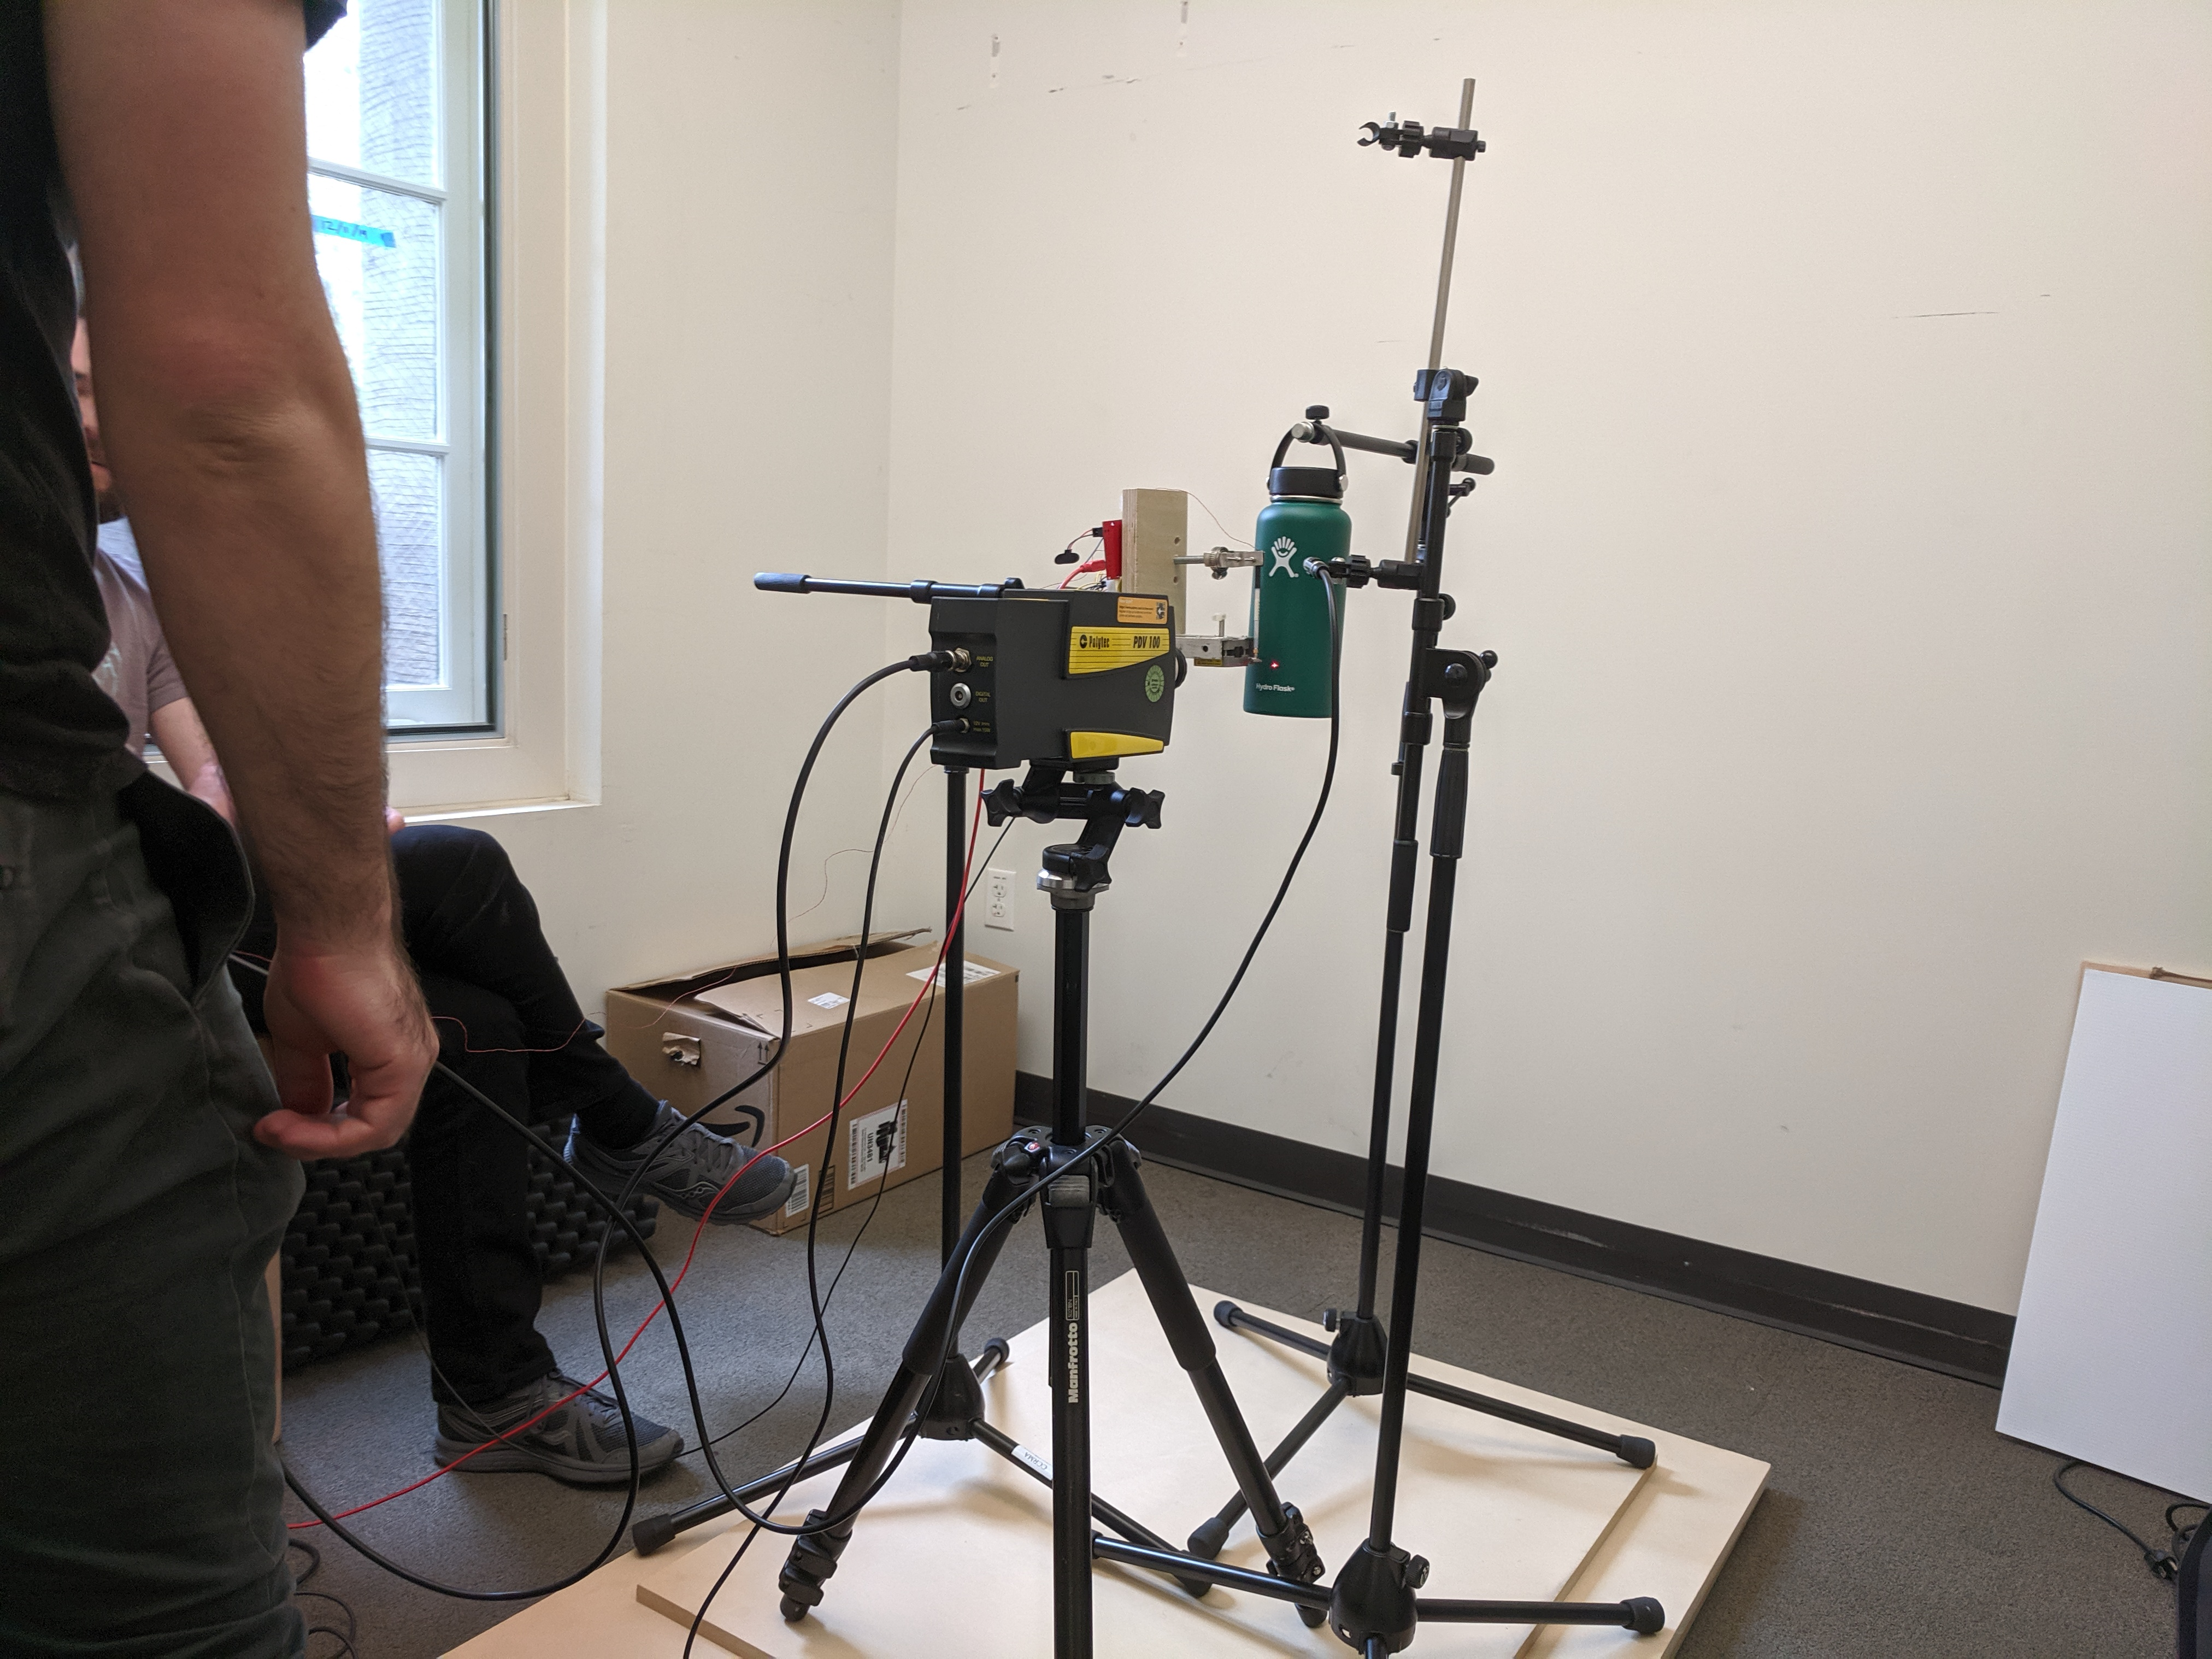
\includegraphics[width=3in]{Figures/hydroflask_measure}
    \caption{\it{Measurement setup for the HydroFlask waterbottle}}
    \label{fig:hydro_measure}
\end{figure}
%
\begin{figure}[!htb]
    \centering
    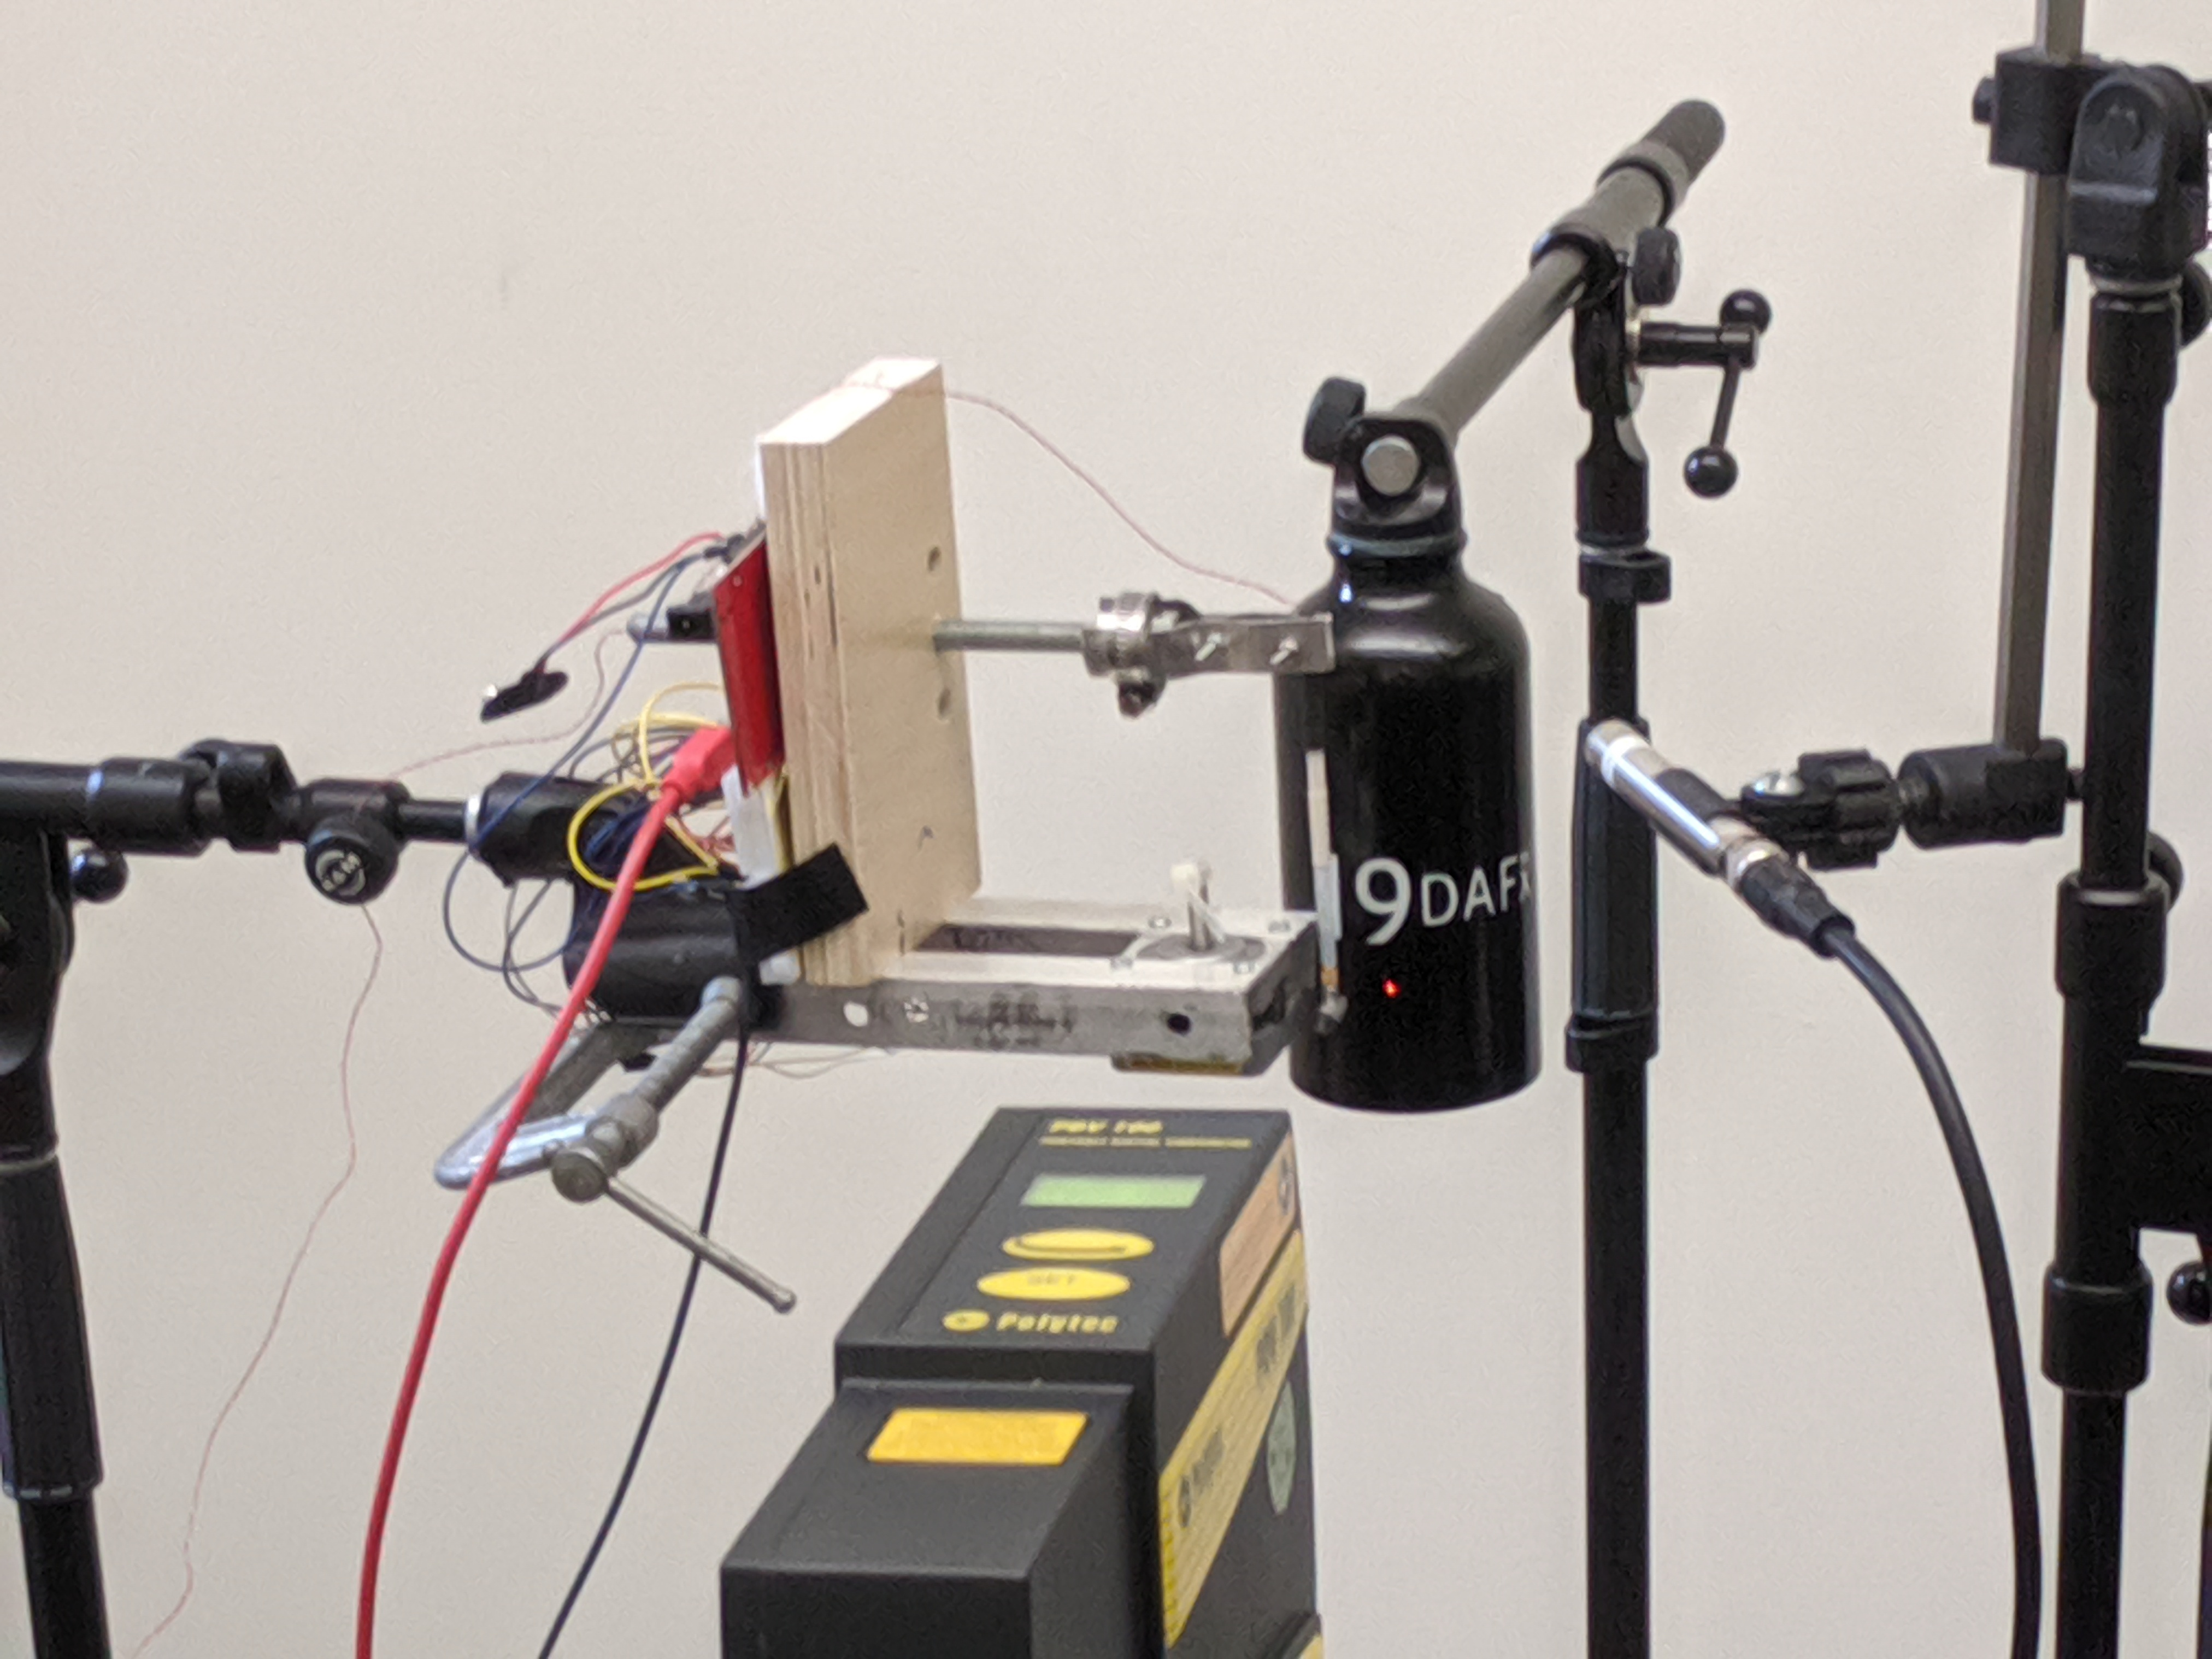
\includegraphics[width=3in]{Figures/dafx_measure}
    \caption{\it{Measurement setup for the DAFx waterbottle}}
    \label{fig:dafx_measure}
\end{figure}

\section{Analysis} \label{sec:analysis}
%
\subsection{Modal Analysis} \label{sec:modal-analysis}
%
Similar to the carillon bells modelled in \cite{canfielddafilou:werner:bellEffects:2017,rau:das:canfielddafilou:carillon:2019},
we can use modal analysis to model the waterbottle sounds as
a sum of exponentially decaying sinusoids.
\begin{equation}
    y(t) = \sum_{m=1}^M \alpha_m e^{j\omega_m t} e^{-t/\tau_m}
    \label{eq:modal-def}
\end{equation}
%
where $\alpha_m$ is the complex amplitude, $\omega_m$ is the mode
frequency, and $\tau_m$ is the decay rate for each mode $m$.
\newline\newline
For modal analysis we use the helper functions
provided by the \texttt{Python} audio signal processing library
\texttt{audio\_dspy}\footnote{\url{https://github.com/jatinchowdhury18/audio_dspy}}.
This process involves the following steps:
\begin{enumerate}
    \item Picking the modal frequencies from the original recording.
    \item Estimate the decay rate of each mode.
    \item Estimate the complex amplitude of each mode.
\end{enumerate}
%
The process is shown in  full in \cref{fig:modal_analysis}.
\newline\newline
For finding the mode frequencies, we use a simple peak picking
algorithm over the Fourier Transform of the original signal.
\newline\newline
For estimating the mode decay rates, we begin by filtering
the signal using a 4th order Butterworth bandpass filter
centered on the mode frequency, with a bandwidth of 30 Hz.
We then apply a Root-Mean-Squared level detector as defined
in \cite{giannoulis2012compressor} to estimate the energy
envelope of the mode. Finally, we use a linear regression
to estimate the slope of the energy envelope (measured in
Decibels).
\newline\newline
After computing the mode frequencies and decay
rate, we can do a simple least squares fit to
estimate the complex amplitude of each mode that
most accurately resynthesizes the original recording.
This process is described in full in \cite{rau:das:canfielddafilou:carillon:2019}.
%
\begin{figure*}
    \centering
    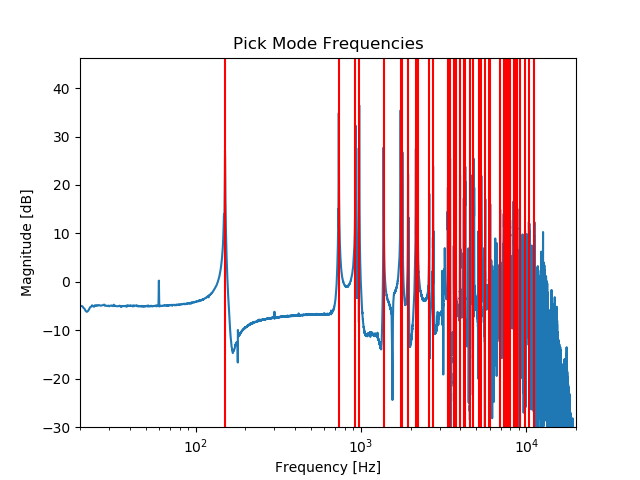
\includegraphics[width=2.25in]{Figures/ModePick_ex}
    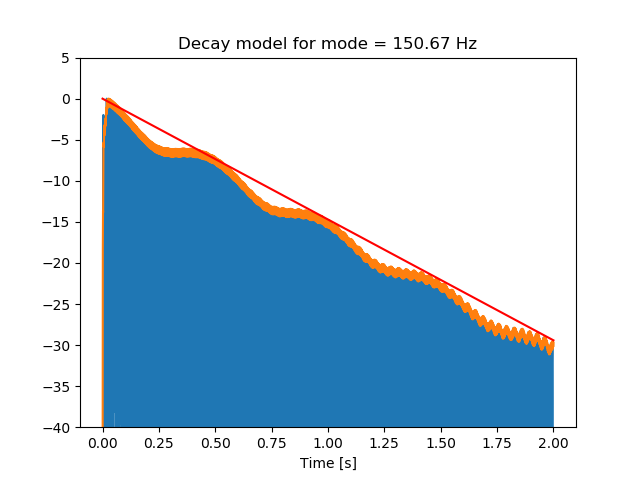
\includegraphics[width=2.25in]{Figures/DecayFit_ex}
    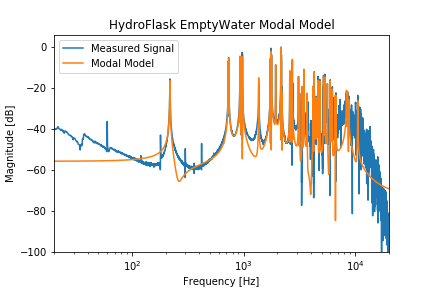
\includegraphics[width=2.25in]{../Figures/HydroFlask/empty}
    \caption{\it{Modal analysis pipeline: (left) picking the mode frequencies,
    (center) estimating the decay rate of a single mode,
    (right) using least-squares to estimate the complex
    amplitudes of the modes that ideally resynthesize the
    original signal.}}
    \label{fig:modal_analysis}
\end{figure*}
%
\subsection{Water Level Analysis} \label{sec:water}
%
Next we examine the how the modal response of the waterbottle
changes as the water level in the waterbottle changes. 
%
\subsubsection{Frequency Variation} \label{sec:water-freq}
%
Measurements od the HydroFlask bottle show that as the water
level increases, the first mode frequency increases, while the
higher modes stay at the same frequency. This makes physical
sense because having a higher water level inside the bottle
effectively decreases the size of the air column inside the
bottle, thereby causing the lowest mode frequency to increase
(@TODO: ask Mark if this is correct).
\newline\newline
@TODO: plot from Matlab (I think Mark has it \dots)
\newline\newline
We can use a cubic spline to model the movement of the first
mode frequency as the water level changes continuously, as
shown in \cref{fig:water-mode-freq}.
%
\begin{figure}[!htb]
    \centering
    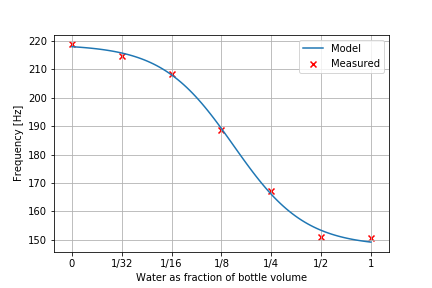
\includegraphics[width=3in]{../Figures/Water_Freq}
    \caption{\it{Variation of the first mode frequency of the HydroFlask
                with the amount of water in the bottle}}
    \label{fig:water-mode-freq}
\end{figure}
%
\subsubsection{Damping Variation} \label{sec:water-damp}
%
Further analysis shows that the damping of the lowest two modes
varies with water level as well. We can similarly model the
variation of the mode decay rates with water level, using a
quartic polynomial to fit the average of decay rates of the first
two modes (see \cref{fig:water-mode-damp}).
%
\begin{figure}[!htb]
    \centering
    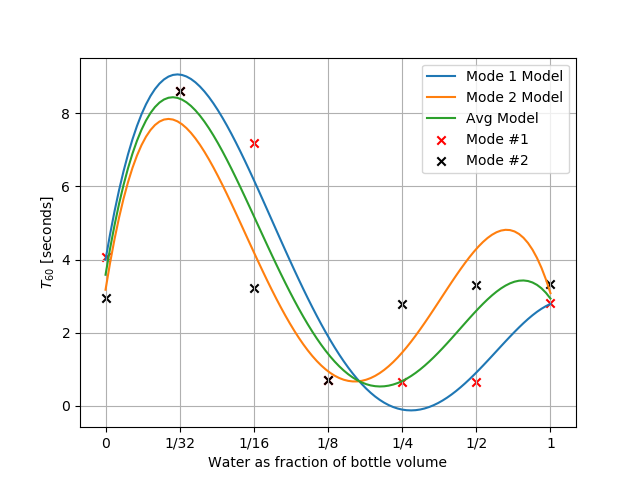
\includegraphics[width=3in]{../Figures/Water_Damping}
    \caption{\it{Variation of the first two modes decay rates
                 with the amount of water in the HydroFlask}}
    \label{fig:water-mode-damp}
\end{figure}
%
\subsection{Sticker Analysis} \label{sec:sticker}
%
Initially, we compared two 32 oz. HydroFlask waterbottles, one
with stickers, one without, and noted that they had different
timbres. We then proceeded to take measurements of the
bottle covered in varying amount of removable stickers. We found
that the mode frequencies remained mostly unchanged with the
addition of stickers, but that the mode dampings had noticeable
variations (see \cref{fig:sticker-mode-damp}).
%
\begin{figure}[!htb]
    \centering
    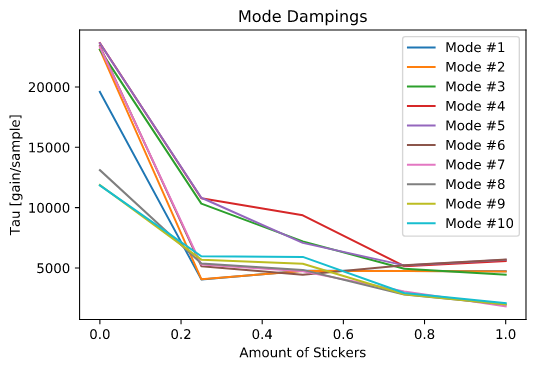
\includegraphics[width=3in]{../Figures/StickerDamping}
    \caption{\it{Variation of the first ten modes decay rates
                 with the amount of stickers on the HydroFlask}}
    \label{fig:sticker-mode-damp}
\end{figure}
%
\subsection{Mode Synthesis} \label{sec:synthesis}
%
For synthesizing the modes we use the Max Matthews
phasor filter, as introduced in \cite{phasorfilter}.
This filter is described by the difference equation:
\begin{equation}
    y_m[n] = \alpha_m x[n] + e^{j\omega_m} e^{-1/\tau_m} y_m[n-1]
    \label{eq:phasor}
\end{equation}
%
where $\tau_m$ is the mode decay rate described above,
$\alpha_m$ is the complex amplitude of the mode, and $\omega_m$
is the mode frequency. This filter structure is known for
having favorable numerical properties, as well as for being
stable regardless of real-time parameter modulation.
%
\section{Results} \label{sec:results}
%
Some general results \dots
%
\subsection{Waterbottle Synthesizer} \label{sec:synth}
%
To demonstrate the musical power of waterbottle synthesis, we have
implemented an 8-voice modal waterbottle synthesizer as an audio
plugin (VST/AU), using the JUCE/C++ framework\footnote{\url{https://github.com/weAreROLI/JUCE}}.
The synthesizer includes controls for the amount of water in the bottle,
the number and placement of stickers on the bottle, and the option To
strike the waterbottle with a variety of objects. Currently, the synthesizer
implements our model of the 32 oz. Wide Mouth HydroFlask, but could easily
be adjusted to model any other waterbottle with similar measurement data.
The source code for this synthesizer is publicly available on
GitHub\footnote{\url{https://github.com/jatinchowdhury18/modal-waterbottles}}.
%
\section{Conclusion} \label{sec:conclusion}
%
In this paper, we have discussed the sythesis of waterbottle acoustics
using modal signal processing techniques. We have described the processes
of making acoustic measurements of the waterbottles, as well as performing
modal analysis, with specific considerations for the amount of water
contained in the bottle, as well as the stickers placed on the exterior
of the bottle. Finally, we have implemented our modal model of a 32 oz.
Wide Mouth HydroFlask bottle as a real-time synthesizer plugin.
\newline\newline
Future research concerns \dots

\section{Acknowledgements}
%
The authors would like to thank Kim Kawsczinski for helping us to contact
the HydroFlask brand.

%\newpage
\nocite{*}
\bibliographystyle{IEEEbib}
\bibliography{references}

\end{document}
